The next Figure \ref{fig:flow} describes the AI, i.e. the MCTS Algorithm module.

\begin{figure}[H]
	\centering
	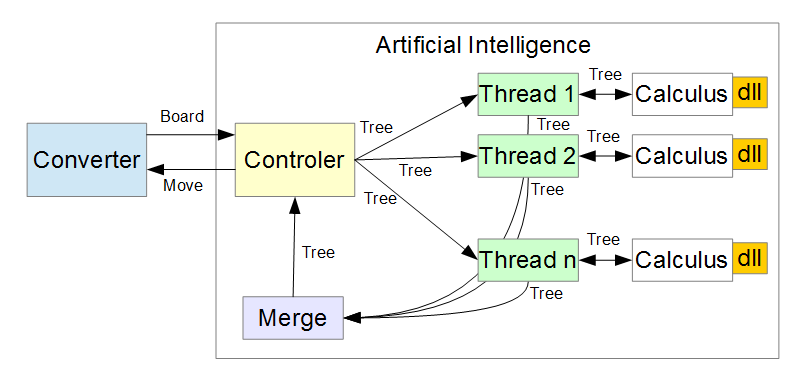
\includegraphics[width=0.80\textwidth]{2General_Architecture/2.3MCTS/AI.png}
	\caption{Block Diagram of Converter}
	\label{fig:flow}
\end{figure}

The converter sends the state of the board to the controler, which creates trees in different threads. Each of these threads computes his tree, getting the possible moves thanks to a set of rules, gathered together in a dynamic link library dll. 

Then, when the calculus is over, the thread hands over the tree to the Merge module. When all threads have done it, the module merges the trees, gathering data in an only tree, that is sent to the controler.

Finally, the controler is able to decide what move to choose and it sent this move to the converter.

